\subsection{Exam: 2022. 06. 20., Exercise 6}

\lineparagraph{Exercise}

Define an ordering of pairs of positive integers as follows. $(a,b) < (c,d)$ holds if and only if
\begin{itemize}
\item $a \cdot{} b < c \cdot{} d$ or
\item $a \cdot{} b < c \cdot{} d$ and $\min(a,b) < \min(c,d)$
\end{itemize}

(For example, $(3,5) < (2,12)$, because $15< 24$ and $(1,20) < (5,4)$, because both products are $20$, but $1 < 4$.) 

The figure below is a binary search tree with using ordering.

\begin{center}
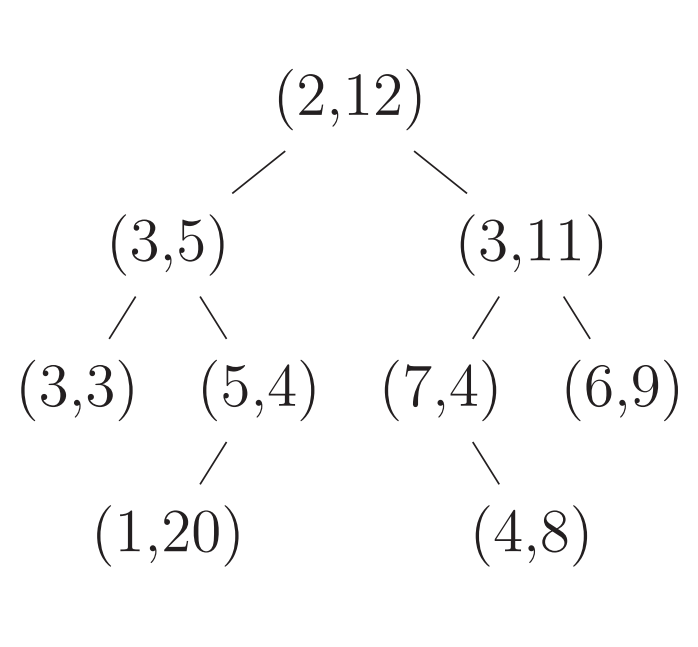
\includegraphics[width=0.5\linewidth]{exams/2022_06_20/06/bintree.png}
\end{center}

\begin{enumerate}[a)]
    \item Insert the element $(6,4)$ into the tree.
    \item Delete the pair $(2,12)$ from the tree obtained in part a).
\end{enumerate}

\lineparagraph{Solution}

Insertion:

\begin{center}
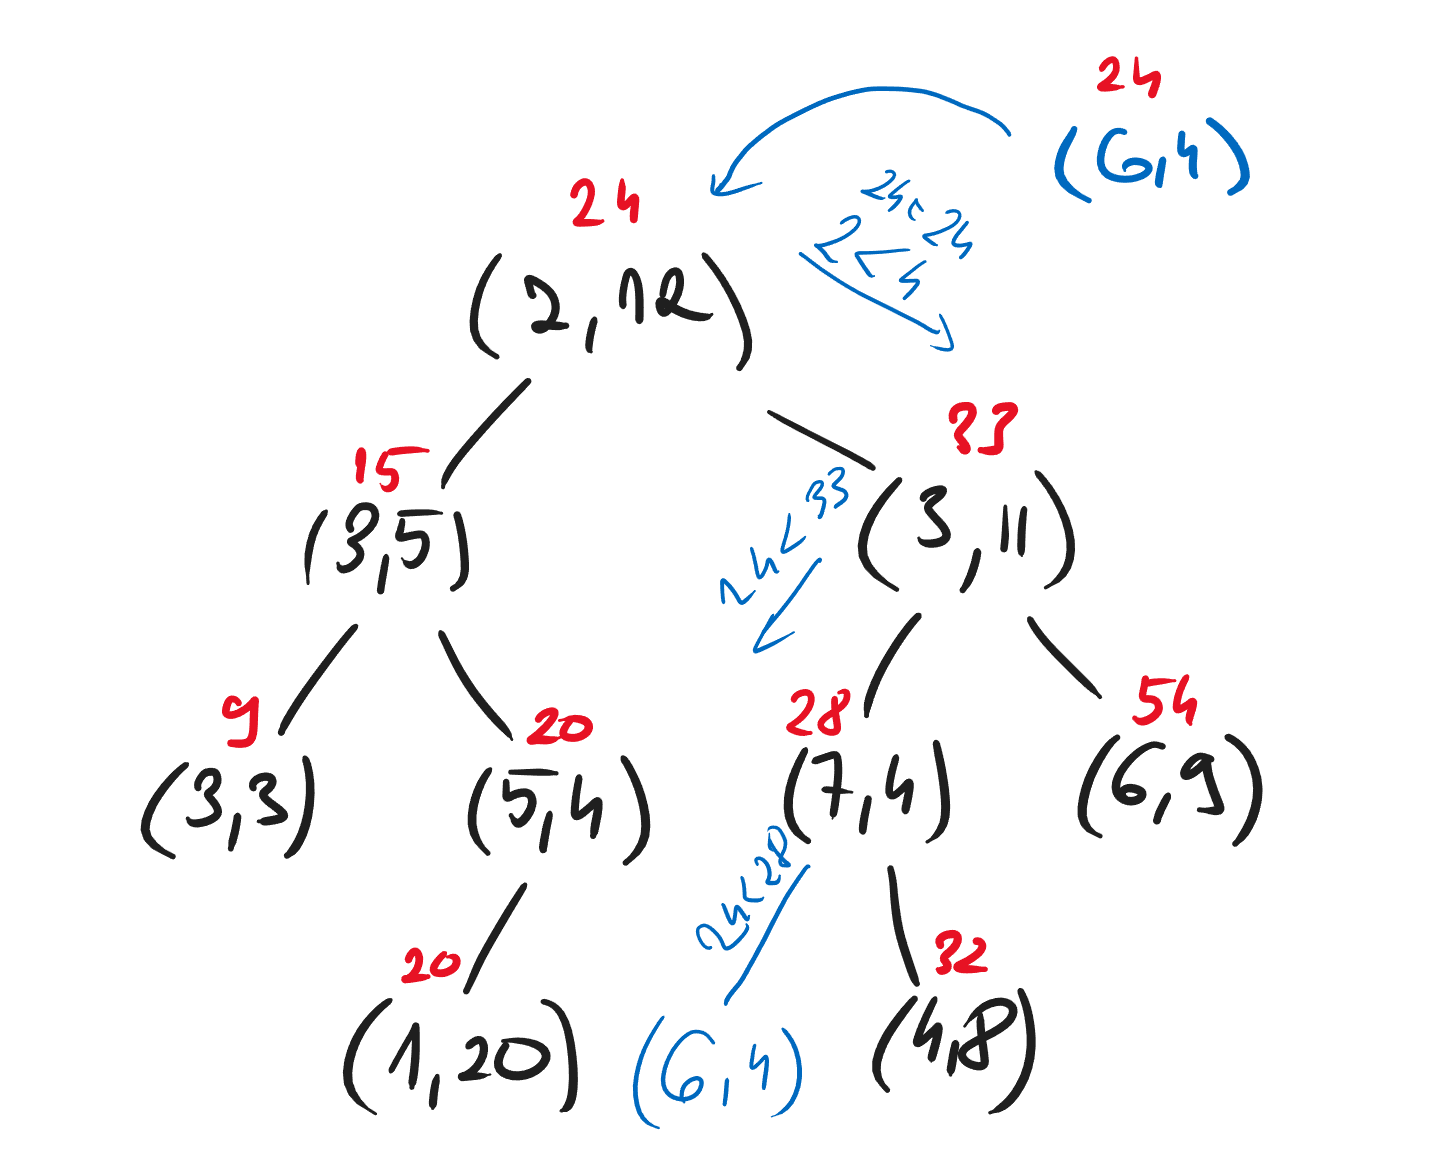
\includegraphics[width=0.5\linewidth]{exams/2022_06_20/06/insert.png}
\end{center}

Deletion:

\begin{itemize}
    \item The minimum element of the right subtree gets put in place of $(2,12)$, which is the $(6,4)$ we just inserted.
    \item You can find the minimum element of the subtree by always navigating to the left, until you reach a leaf.
\end{itemize}

\begin{center}
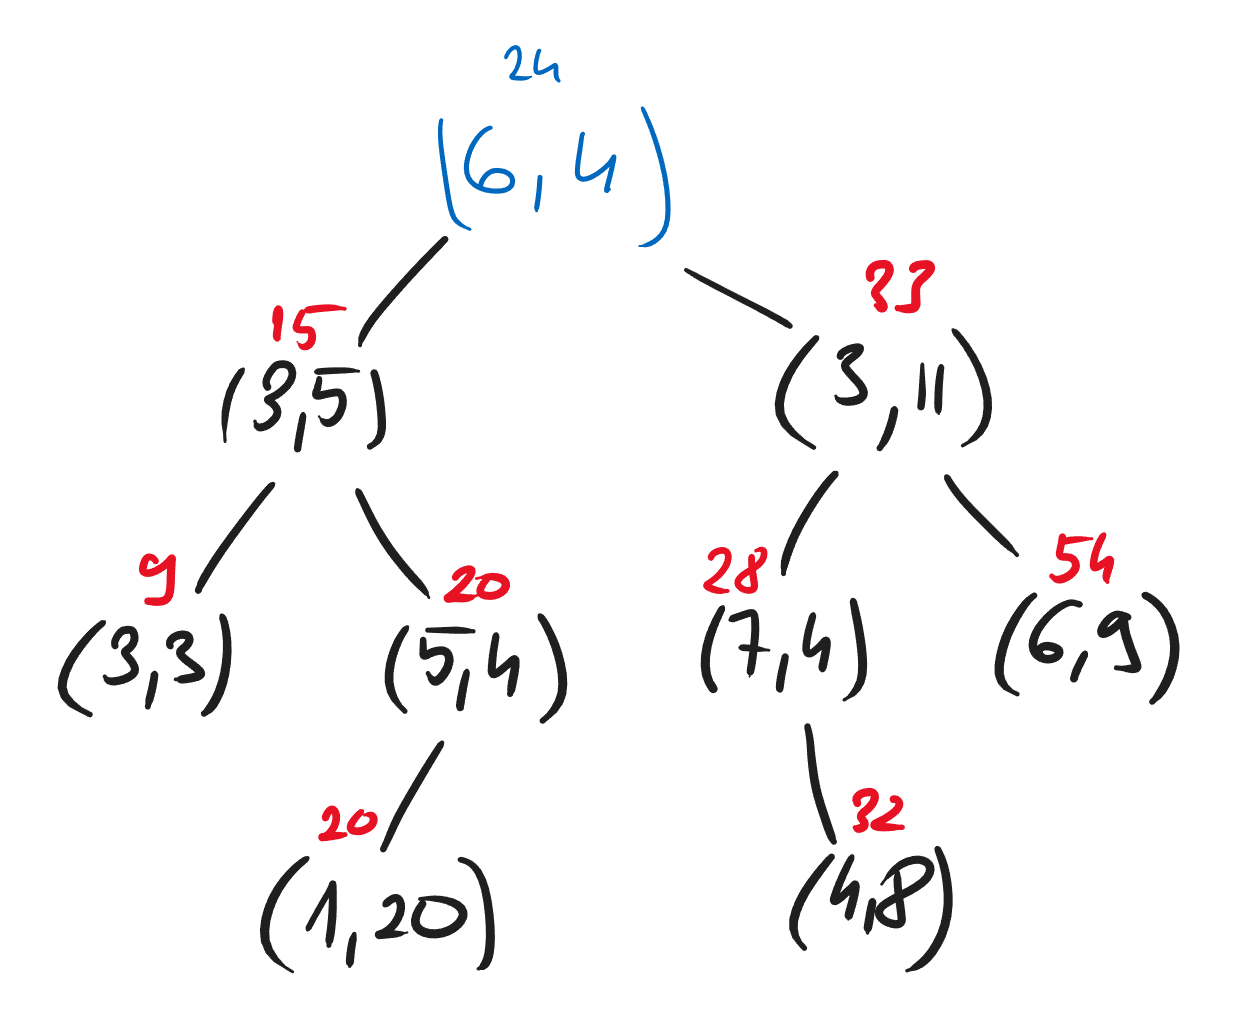
\includegraphics[width=0.5\linewidth]{exams/2022_06_20/06/delete.png}
\end{center}
